\begin{center}
    \begin{figure}[H]
        \centering

        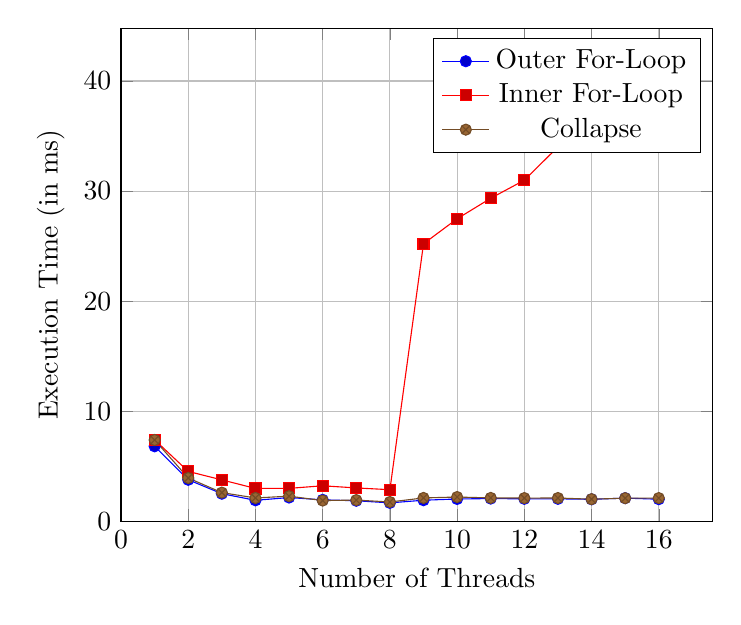
\begin{tikzpicture}
            \begin{axis}[
                title={},
                width=0.75\textwidth,
                xlabel={Number of Threads},
                ylabel={Execution Time (in ms)},
                xmin=0,
                ymin=0,
                grid=major
            ]
                \addplot coordinates {
                    (1,6.8133)(2,3.772)(3,2.5074)(4,1.9063)(5,2.1592)(6,1.9498)(7,1.86735)(8,1.67335)(9,1.91465)(10,2.0285)(11,2.0644)(12,2.04225)(13,2.0411)(14,1.9984)(15,2.10485)(16,2.00745)
                };
                \addlegendentry{Outer For-Loop}

                \addplot coordinates {
                    (1,7.39955)(2,4.5312)(3,3.76235)(4,2.98635)(5,2.99115)(6,3.22585)(7,3.03185)(8,2.87065)(9,25.2141)(10,27.4829)(11,29.348)(12,30.9892)(13,34.0131)(14,39.4454)(15,40.0405)(16,40.7224)
                };
                \addlegendentry{Inner For-Loop}       

                \addplot coordinates {
                    (1,7.38385)(2,3.9323)(3,2.60535)(4,2.11995)(5,2.28335)(6,1.88385)(7,1.92715)(8,1.75435)(9,2.12325)(10,2.2048)(11,2.12435)(12,2.10905)(13,2.11495)(14,2.00945)(15,2.1006)(16,2.1095)
                };
                \addlegendentry{Collapse}
            \end{axis}
        \end{tikzpicture}
        \caption{HSV Performance Tests dice.png}
    \end{figure}
\end{center}